Z powyższych własności można wyciągnąć parę przykładów zbiorów przeliczalnych. Jednym z~nich jest \( \natural^2 \).
\newpage
\begin{lemma}
    Zbiór \( \natural^2 \) jest przeliczalny.
\end{lemma}
\begin{proof}
    Definiujemy bijekcję \( \pi : \natural^2 \rightarrow \natural \) następująco:
    \begin{figure}[H]
        \centering
        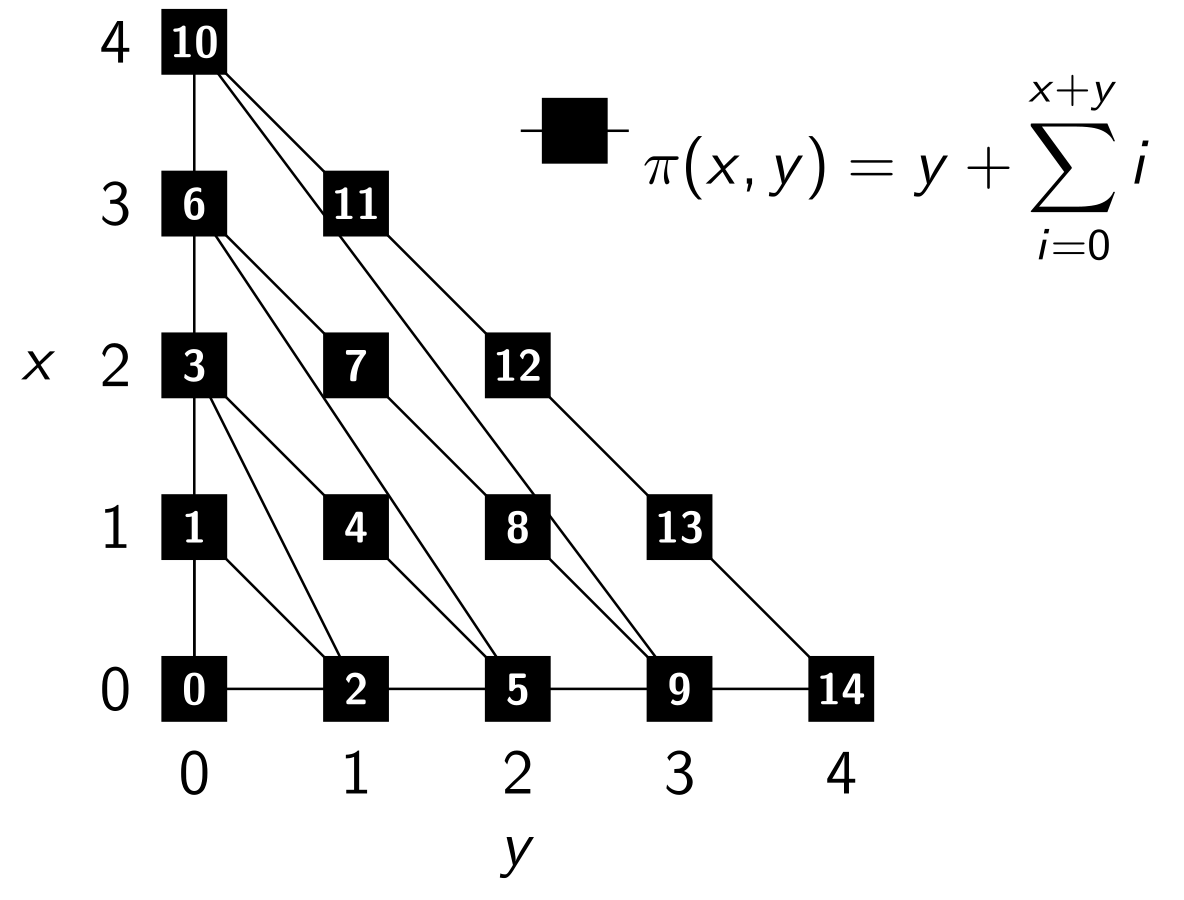
\includegraphics[height=0.5\textwidth]{chapters/mfi/countable/pairing-function}
        \caption{Pairing-function, autor: MartinThoma, Wikimedia Commons, \url{https://commons.wikimedia.org/wiki/File:Pairing-function.svg}}
    \end{figure}
\end{proof}

Można poszukać też innych przykładów:
\begin{lemma}
    Zbiory liczb całkowitych i wymiernych są przeliczalne.
\end{lemma}
\begin{proof}
    Korzystamy z punktu 6 Lematu~\ref{lemma:countable-properties}. Zbiory \( \integer = \natural \times \natural/\!\simeq \) oraz \( \rational = \integer \times \integer^{*}/\!\simeq \) są~rozkładami zbiorów przeliczalnych.
\end{proof}